\documentclass{article}
\usepackage{tikz}
\usetikzlibrary{graphs, graphs.standard, quotes}

\begin{document}

\textbf{PD-L1 Model}, relating some key factors for tumor progression\\
Shaded nodes compose the features \( X \). Tumor Growth (thick circle on the right) is the endpoint \( y \).

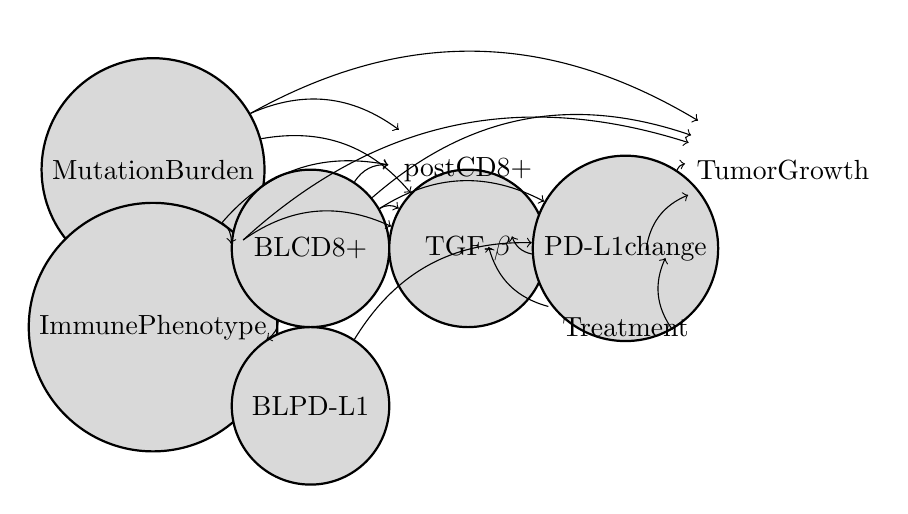
\begin{tikzpicture}[every node/.style={circle, draw, thick, minimum size=20mm}]
    % Define nodes
    \node[fill=gray!30] (mutation) at (-4, 0) {Mutation\\Burden};
    \node[fill=gray!30] (immune) at (-4, -2) {Immune\\Phenotype};
    \node[fill=gray!30] (blcd8) at (-2, -1) {BL\\CD8+};
    \node[fill=gray!30] (blpd1) at (-2, -3) {BL\\PD-L1};
    \node[fill=gray!30] (tgfbeta) at (0, -1) {TGF-\(\beta\)};
    \node[fill=gray!30] (pd1change) at (2, -1) {PD-L1\\change};
    \node[draw=none] (postcd8) at (0, 0) {post\\CD8+};
    \node[draw=none] (tumor) at (4, 0) {Tumor\\Growth};
    \node[draw=none] (treatment) at (2, -2) {Treatment};

    % Draw edges
    \path[->]
        (mutation) edge[bend left] (tgfbeta)
        (mutation) edge[bend left] (postcd8)
        (mutation) edge[bend left] (tumor)
        (immune) edge[bend left] (tgfbeta)
        (immune) edge[bend left] (postcd8)
        (immune) edge[bend left] (tumor)
        (immune) edge[bend left] (blcd8)
        (immune) edge[bend left] (blpd1)
        (blcd8) edge[bend left] (tgfbeta)
        (blcd8) edge[bend left] (postcd8)
        (blcd8) edge[bend left] (tumor)
        (blcd8) edge[bend left] (pd1change)
        (blpd1) edge[bend left] (pd1change)
        (pd1change) edge[bend left] (postcd8)
        (pd1change) edge[bend left] (tumor)
        (pd1change) edge[bend left] (treatment)
        (treatment) edge[bend left] (postcd8)
        (treatment) edge[bend left] (tumor);
\end{tikzpicture}

\end{document}